\documentclass[MScDSA]{uccthesis}

\title{The \texttt{uccthesis} Class}
\author{M.\,R.\,C. van Dongen}
\supervisor{Dr Who}
\secondreader{Dr Who}
\date{\today}

\newcommand*{\COMMAND}[1]{\texttt{\textbackslash #1}}
\newcommand*{\COMMANDWITHARGUMENT}[2]{\texttt{\textbackslash #1}\{#2\}}

\addbibresource{mybib.bib}% should be in preamble

\abstract{%
   This document describes the \texttt{uccthesis} class.
}

%\dedication{%
%   Your dedication here.
%}

%\acknowledgement{%
%   Your acknowledgement here.
%}

\renewcommand\addToFrontMatter[0]{%
}

\begin{document}
   \chapter{Introduction}
      This chapter explains the \texttt{uccthesis} class,
       the main purpose of which is to write a thesis
       with minimal configuration.

   \section{Thesis Structure}
      A typical thesis consists of
       \emph{front matter},
       \emph{main matter}, and
       \emph{back matter}.
      The front matter of
        of typical document consists of
       (1)~a title page with title back page,
       (2)~an abstract,
       (3)~a declaration page,
       (4)~an optional acknowledgement page,
       (5)~an optional dedication page, and
       (6)~a table of contents,
       (7)~a list of tables, and
       (8)~a list of figures.
      The frontmatter is inserted \emph{automatically}.
      The back matter typically
       consists of the bibliography.
      Any other back matter should be typeset explicitly.

      The commands `\COMMAND{declaration}' and
       `\COMMAND{dedication}' may be used to
       include a declaration or a dedication.
      However, there is no need to use these commands.

      The main matter of the document
       starts by writing \COMMANDWITHARGUMENT{begin}{document}.
      Additional material may be added
       to the document's front matter by \emph{redefining} the command
       \label{addToFrontMatter}
       `\COMMAND{addToFrontMatter[0]}'.
      This may be useful if you wish to include
       additional lists of things to the document front matter.
      Any commands which are defined by this command
       are inserted before the first chapter.
      You should use the `\COMMAND{renewcommand}'
       command to redefine the command
       `\COMMAND{addToFrontMatter}'.

   \section{Class Options}
      The \texttt{uccthesis}
       class is built on top of the \texttt{book}%
       ~\parencite{Lamport:94} class.
      The options
       `\texttt{a4paper}',
       `\texttt{openright}',
       `\texttt{titlepage}', and
       `\texttt{fleqn}'
       are automatically passed to the \texttt{book} class by default.
      The `\texttt{draft}' option is only passed to
       the `\texttt{book}' class if you provide the option
       as an option of the \texttt{uccthesis} class.
      Using the option
       results in displaying the word `Draft' on the titlepage.
      Table~\ref{tab:options} lists the remaining document options
       and default values.
      \begin{table}[tbp]
      \begin{tabular}{lll}
        \toprule
        \textbf{Option}   & \textbf{Default} & \textbf{Description}
      \\\midrule
        \textbf{10pt}     &     & Set point size to 10\,pt
      \\\textbf{11pt}     &     & Set point size to 11\,pt
      \\\textbf{12pt}     & on  & Set point size to 12\,pt
      \\\textbf{oneside}  & on  & Enforce onesided pages
      \\\textbf{twoside}  &     & Enforce twosided pages
      \\\textbf{singlespacing} & on & Set line spacing to single spacing
      \\\textbf{onehalfpacing} & off & Discouraged: set line spacing to $1.5$ spacing
      \\\textbf{doublespacing} & off & Discouraged: set line spacing to double spacing
      \\\textbf{draft}    &     & Set draft option
      \\\midrule
        \multicolumn{3}{r}{\textbf{Sets Degree to}}
      \\\midrule
        \textbf{BScCS}    &     & BSc Computer Science
      \\\textbf{BScDSA}   &     & BSc Data Science and Analytics
      \\\textbf{DHIT}     &     & BA Digital Humanities and Information Technology
      \\\textbf{MScCS}    &     & MSc Computing Science
      \\\textbf{MScDSA}   &     & MSc Data Science and Analytics
      \\\textbf{MScIM}    &     & MSc Interactive Media
      \\\textbf{MScResearch} &  & MSc Computer Science (Research)
      \\\textbf{PhD}      &     & PhD Computer Science
      \\\midrule
        \textbf{ManyFigures}   &    & Increase width of figure numbers in \texttt{lof}
      \\\textbf{ManyTables}    &    & Increase width of table numbers in \texttt{lot}
      \\\textbf{ManySections}  &    & Increase width of section numbers in \texttt{toc}
      \\\textbf{ManySubsections}&    & Increase width of subsection numbers in \texttt{toc}
      \\\textbf{final}    & on  & Set draft option off
      \\\textbf{lot}      & on  & Include a list of tables
      \\\textbf{nolot}    &     & Do not include a list of tables
      \\\textbf{lof}      & on  & Include a list of figures
      \\\textbf{nolof}    &     & Do not include a list of figures
      \\\textbf{*}        & N/A & Option is passed to \texttt{book} class
      \\\bottomrule
      \end{tabular}
      \caption[Class options of \protect\texttt{uccthesis} class.]
              {\label{tab:options}Class options of \protect\texttt{uccthesis} class.
               Most options are off by default.
               The word `on' in the column `Default' is used
                if and only if the option is on by default.
               None of the options
                \texttt{BScCS}, \texttt{BScDSA}, \texttt{DHIT},
                \texttt{MScCS}, \texttt{MScDSA}, \texttt{MScIM}, \texttt{MScResearch}, and
                \texttt{PhD}
                is a default option.
               At least one of these opions must be provided.
               Failing to provide them will result in an error.}
      \end{table}
      The only allowed options to change the point size are
       \texttt{10pt},
       \texttt{11pt}, and
       \texttt{12pt}.
      Other options related to the point size are not supported.
      The options
       \texttt{a5paper},
       \texttt{b5paper},
       \texttt{letterpaper},
       \texttt{legalpaper},
       \texttt{executivepaper}, and
       \texttt{landscape}
       are also not supported.

      Please note that a table of contents,
       a list of tables, and
       a list of figures are included \emph{by default.}
      Including a list of tables and list of figures
       can be turned off with the options
       `\texttt{nolot}' and `\texttt{nolof}'.

   \section{Styles}

      The following style files are automatically loaded by
       the class:
       \texttt{amsthm},
       \texttt{amsmath},
       \texttt{babel},
       \texttt{beramono},
       \texttt{biblatex},
       \texttt{booktabs},
       \texttt{calc},
       \texttt{chngpage},
       \texttt{fancyhdr},
       \texttt{fontenc},
       \texttt{fourier},
       \texttt{graphicx}.
       \texttt{inputenc},
       \texttt{microtype},
       \texttt{minitoc},
       \texttt{pgfplots},
       \texttt{setspace},
       \texttt{textcase},
       \texttt{tikz},
       \texttt{url}, and
       \texttt{xcolor},

   \section{Bibliography Style}

      The bibliography style is hardcoded
       with \texttt{biblatex}~\parencite{biblatex}, which
       is automatically loaded so you can
       distinguish between
       \emph{parenthetical citations}: \parencite{biblatex}, and
       \emph{textual citations}:\textcite{biblatex}.
      The former kind of citations may be obtained
       with the command \COMMAND{parencite}.
      The latter citations may be obtained
       with the command \COMMAND{textcite}.
      You can force an uppercase letter in a ``Von'' part by
       capitalising the first letter of these commands:
       \COMMAND{Parencite} and
       \COMMAND{Textcite}.
      For example,
       with the parenthetical version this gives you
       `\Textcite{LAF}' as opposed to `\textcite{LAF}'.
      More details may be found in \Textcite{LAF}.
      Any attempt to redefine the bibliography style is ignored.
      \emph{Note that the \texttt{biblatex} package
             only lets you put the \COMMAND{bibliography}
             command in the document preamble.}

      Since the bibliography depends on \texttt{biblatex},
       users should refrain from using the \COMMAND{cite} command.

      The \texttt{biblatex} package uses \texttt{biber} as the back-end.
      When citations have changed or the bibliography has changed,
       they should run the \texttt{biber} command (not \texttt{bibtex})
       on the base name of they main thesis source file.

   \section{Implementation Details}

      The implementation is relatively simple.
      The code for the titlepage is borrowed
       from \texttt{arsclassica}~\Parencite{arsclassica}
      A few macros are from
       \texttt{arsclassica}~\Parencite{arsclassica} and
       \texttt{classicthesis}~\Parencite{classicthesis}
      The code to typeset the abstract is from
       the \texttt{book}~\Parencite{Lamport:94} class.
      The code for the pagestyle for twosided documents
       is based on the \texttt{fancyhdr} manual~\Parencite{fancyhdr}.

      The author of the thesis is defined with
       the \COMMAND{author} command.
      The name of the supervisor is defined with
       the \COMMAND{supervisor} command.
      The name of the second reader is defined with
       the \COMMAND{secondreader} command.

   \chapter{Example}

      Figure~\ref{fig:example}
       depicts a minimal example of how to use the \texttt{uccthesis} class.
      \begin{figure}[hbtp]
      \hrule
      \vspace{0.5em}
\begin{scriptsize}
\begin{verbatim}
% Thesis for MSc Computing Science with default style.
%\documentclass[MScCS]{uccthesis}
% The following uses all default options.
% \documentclass[MScDSA,lof,lot,12pt,oneside,singlespacing,final]{uccthesis}
% Other examples:
% \documentclass[MScCS,nolof,nolot,11pt,twoside,singlespacing,draft]{uccthesis}
 \documentclass[MScIM,12pt]{uccthesis}
% \documentclass[BSc,12pt]{uccthesis}

\addbibresource{mybib.bib} % bibliography must be defined in preamble

\title{How I got my MSc}
\author{Student's Name}
\supervisor{Supervisor's Name}
\secondreader{Second Reader's Name}
\date{\today} % Student should define the actual date

\abstract{Abstracts should be short.}
\dedication{This thesis is dedicated to mum.}
%\acknowledgement{Your acknowledgement here.}

\renewcommand\addToFrontMatter[0]{%
}

\begin{document}
   \chapter{Introduction}
      \ldots
   \chapter{Notation}
      \ldots
   \chapter{Conclusions}
      \ldots
   % start backmatter
   \backmatter
   % Print the bibliography
   \printbibliography
\end{document}
\end{verbatim}
\end{scriptsize}
      \hrule
      \caption{\label{fig:example}Using the \protect\texttt{uccthesis} class.}
      \vspace{0.5em}
      \hrule
   \end{figure}

      The following
       demonstrates how to include an external picture.
\begin{scriptsize}
\begin{verbatim}
The following
 demonstrates how to include an external picture.
\begin{figure}[hbtp]
\hrule
\vspace{0.5em}
\centering
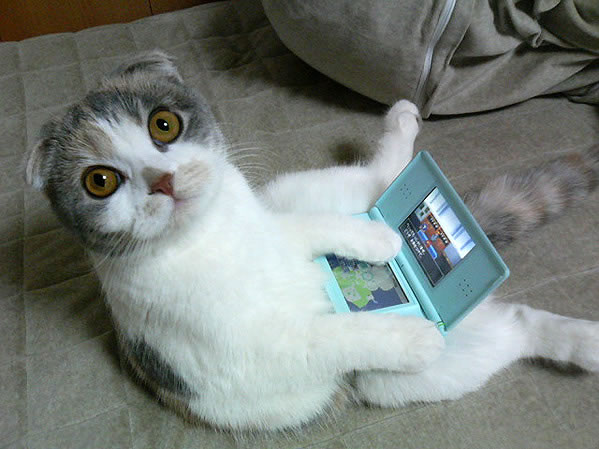
\includegraphics[width=0.95\textwidth]{Figures/jpgpic.jpg}
\vspace{0.5em}
\hrule
\caption{\label{fig:including@a@picture}Including an external picture.}
\vspace{0.5em}
\hrule
The result is depicted in Figure~\ref{fig:including@a@picture}
\end{verbatim}
\end{scriptsize}
      The result is depicted in Figure~\ref{fig:including@a@picture}

      \begin{figure}[hbtp]
      \hrule
      \vspace{0.5em}
      \centering
      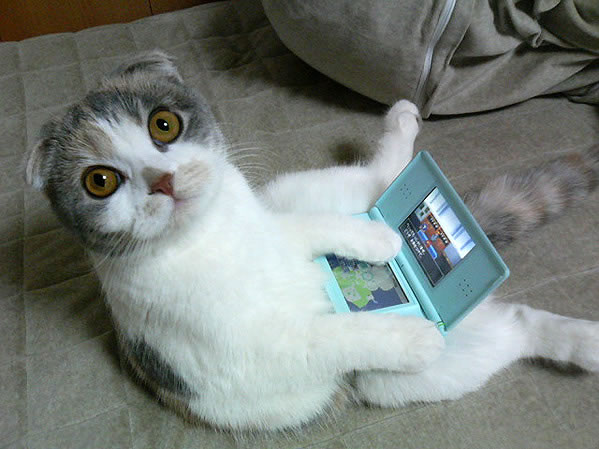
\includegraphics[width=0.95\textwidth]{Figures/jpgpic.jpg}
      \vspace{0.5em}
      \hrule
      \caption{\label{fig:including@a@picture}Including an external picture.}
      \vspace{0.5em}
      \hrule
   \end{figure}

\chapter{Bugs and Requests for Features}

   Bugs and requests for features
    may be reported by email to \url{dongen@cs.ucc.ie}.
   When reporting bugs, please describe
    the bug as well as providing a \emph{minimal} example.

%
%
\backmatter
%
%
   \printbibliography
\end{document}
